\documentclass[class=minimal,border=0pt]{standalone}

\usepackage{tikz}

\usetikzlibrary{arrows,shapes}
\tikzstyle{erlang} = [draw=gray!90, dashed,rectangle, minimum height=4em, minimum width=8em]
\tikzstyle{expo} = [draw, fill=orange!25,draw=orange!80, circle, minimum height=2em]
\tikzstyle{expo2} = [draw, fill=blue!25,draw=blue!80, circle, minimum height=2em]
\tikzstyle{nothing} = [coordinate]

\begin{document}

  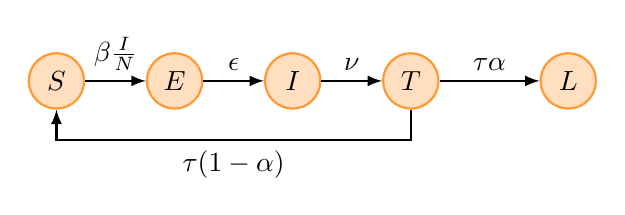
\begin{tikzpicture}[node distance=1.5cm, auto, >=latex, thick]

  % We need to set at bounding box first. Otherwise the diagram
    % will change position for each frame.
    \node [expo] (sain) {$S$};
    \node [expo, right of=sain] (expose) {$E$};
    \node [expo, right of=expose] (infecte) {$I$};
    \node [expo, right of=infecte] (immunise) {$T$};
    \node [expo, right of=immunise,node distance=2cm] (longue) {$L$};

% Once the nodes are placed, connecting them is easy. 
    \draw [->] (sain) -- node {$\beta\frac{I}{N}$} (expose);
    \draw [->] (expose) -- node{$\epsilon$}(infecte);
    \draw [->] (infecte) -- node{$\nu$}(immunise);
    \draw [->] (immunise) -- node{$\tau\alpha$}(longue);
    \draw [->] (immunise) -- +(0,-0.75) -| node[near start,below] {$\tau(1-\alpha)$}(sain);


  \end{tikzpicture}

\end{document}
